\documentclass{standalone}
\usepackage{tikz}
\usepackage{scalerel}

% \usetikzlibrary{positioning,chains,arrows}
\begin{document}
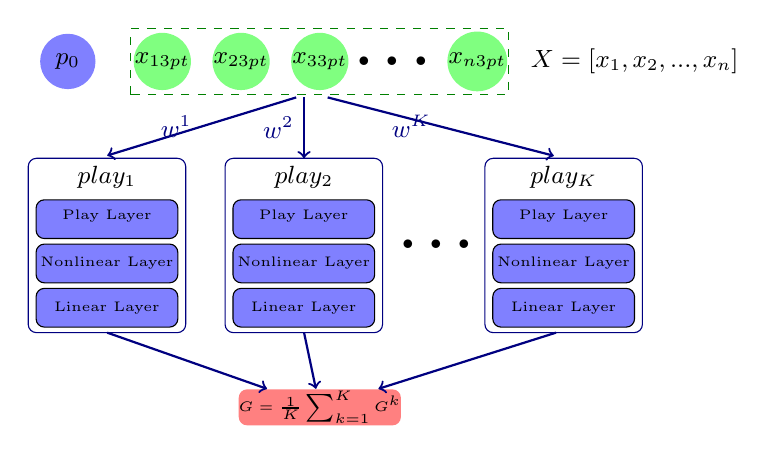
\begin{tikzpicture}[font=\small]
                       
    \tikzstyle{neuron}=[circle,fill=black!25,minimum size=20pt,inner sep=0pt]
    \tikzstyle{input neuron}=[neuron, fill=green!50];
    \tikzstyle{hidden neuron}=[neuron, fill=blue!50];
    \tikzstyle{activation neuron}=[neuron, fill=blue!50, rectangle, rounded corners=3pt, minimum size=13pt];
    \tikzstyle{play output neuron}=[neuron, fill=red!50, rectangle, rounded corners=3pt, minimum size=13pt];
    %% draw neurons
    % \draw (0.2, 0.7) node [] {Multiple Play};
    \node[hidden neuron] at (-0.2,0) {$p_0$};

    \foreach \x in {1,2,3} {
        \node[input neuron] (x_\x) at (\x, 0) {$x_{\scaleto{\x}{3pt}}$};
    }
    \node[input neuron] (x_n) at (5,0) {$x_{\scaleto{n}{3pt}}$};
    \path (x_3) -- (x_n) node[midway,scale=2,font=\bfseries] {\dots};
    \draw[dashed,thin,green!50!black] (0.6,-12pt) rectangle (5.4, 12pt);
    \node[] (input) at (2.8,-10pt) {}; % make anchor here
    \node[] at (7, 0) {$X=[x_1,x_2,...,x_n]$};
    
    \begin{scope}[xshift=-20]
    \foreach \x / \idx in {0/1,2.5/2} {
        \draw[thick,solid,rounded corners=3pt,thin,blue!50!black] (\x,-35pt) rectangle (\x+2, -98pt);
        % \node[] (play_\idx) at (\x+1, -35pt);
        \node[] at (\x+1, -42pt) {$play_\idx$};
        
        \draw[solid,rounded corners=3pt,thin,fill=blue!50!white] (\x+0.1,-50pt) rectangle (\x+1.9, -64pt);
        \node[]  at (\x+1,-56pt) {\tiny Play Layer};
        \draw[solid,rounded corners=3pt,thin,fill=blue!50!white] (\x+0.1,-66pt) rectangle (\x+1.9, -80pt);
        \node[]  at (\x+1,-73pt) {\tiny Nonlinear Layer};
        \draw[solid,rounded corners=3pt,thin,fill=blue!50!white] (\x+0.1,-82pt) rectangle (\x+1.9, -96pt);
        \node[]  at (\x+1,-89pt) {\tiny Linear Layer};
    }
    
    \draw[thick,solid,rounded corners=3pt,thin,blue!50!black] (5.8,-35pt) rectangle (7.8, -98pt);
    \node[] (play_k) at (6.8, -35pt) {};
    \node[] at (6.8, -42pt) {$play_K$};
    \draw[solid,rounded corners=3pt,thin,fill=blue!50!white] (5.9,-50pt) rectangle (7.7, -64pt);
    \node[]  at (6.8,-56pt) {\tiny Play Layer};
    \draw[solid,rounded corners=3pt,thin,fill=blue!50!white] (5.9,-66pt) rectangle (7.7, -80pt);
    \node[]  at (6.8,-73pt) {\tiny Nonlinear Layer};
    \draw[solid,rounded corners=3pt,thin,fill=blue!50!white] (5.9,-82pt) rectangle (7.7, -96pt);
    \node[]  at (6.8,-89pt) {\tiny Linear Layer};
    \end{scope}

    \path (4.3,-66pt) -- (4.8, -66pt) node[midway,scale=2,font=\bfseries] {\dots};

    \draw [->,color=blue!50!black,thick] (2.7,-13pt) to node [left,color=blue!50!black] {$w^1$} (0.3,-34pt);
    \draw [->,color=blue!50!black,thick] (2.8,-13pt) to node [left,color=blue!50!black] {$w^2$} (2.8,-35pt);
    \draw [->,color=blue!50!black,thick] (3.1,-13pt) to node [left,color=blue!50!black] {$w^K$} (play_k);
    
    \node[play output neuron] (output) at (3, -125pt) {\tiny $G=\frac{1}{K}\sum_{k=1}^{K}G^{k}$};
    
    \draw [->,color=blue!50!black,thick] (0.3,-98pt) to node [left,color=blue!50!black] {} (output);
    \draw [->,color=blue!50!black,thick] (2.8,-98pt) to node [left,color=blue!50!black] {} (output);
    \draw [->,color=blue!50!black,thick] (6.,-98pt) to node [left,color=blue!50!black] {} (output);
\end{tikzpicture}
\end{document}

